\documentclass[11pt]{article}
\usepackage[a4paper, margin=2.3cm]{geometry}
\usepackage[T1]{fontenc}
\usepackage{lmodern}
\usepackage{microtype}
\usepackage{graphicx}
\usepackage{float}
\usepackage{amsmath, amssymb}
\usepackage{xcolor}
\usepackage{booktabs}
\usepackage{array}
\usepackage{enumitem}
\usepackage{listings}
\usepackage{fancyhdr}
\usepackage{titlesec}
\usepackage[most]{tcolorbox}
\usepackage{tikz}
\usetikzlibrary{shapes.geometric, arrows.meta, positioning, fit, backgrounds, calc}
\usepackage[colorlinks=true, linkcolor=navy, urlcolor=navy]{hyperref}

% ---------- colours ----------
\definecolor{navy}{HTML}{1F3A5F}
\definecolor{teal}{HTML}{1B7F79}
\definecolor{amber}{HTML}{C77D0A}
\definecolor{brick}{HTML}{B03A2E}
\definecolor{leaf}{HTML}{2E7D32}
\definecolor{paper}{HTML}{F6F7F9}
\definecolor{codebg}{HTML}{F4F4F0}

% ---------- layout ----------
\setlength{\parskip}{0.55em}
\setlength{\parindent}{0pt}
\renewcommand{\arraystretch}{1.25}
\setlist{itemsep=0.2em, topsep=0.3em}
\pagestyle{fancy}
\fancyhf{}
\fancyhead[L]{\small\textcolor{navy}{Lab 6 -- MBIST \& Two-Stage LEC}}
\fancyhead[R]{\small R Sarang -- EC23I2015}
\fancyfoot[C]{\small\thepage}
\renewcommand{\headrulewidth}{0.4pt}
\titleformat{\section}{\Large\bfseries\color{navy}}{\thesection}{0.6em}{}
\titleformat{\subsection}{\large\bfseries\color{teal}}{\thesubsection}{0.6em}{}
\titleformat{\subsubsection}{\normalsize\bfseries\color{navy}}{\thesubsubsection}{0.6em}{}

% ---------- code ----------
\lstdefinestyle{lab}{
  backgroundcolor=\color{codebg}, basicstyle=\ttfamily\footnotesize,
  commentstyle=\color{leaf}, keywordstyle=\color{brick}\bfseries,
  numbers=left, numberstyle=\tiny\color{gray}, numbersep=6pt,
  breaklines=true, keepspaces=true, showstringspaces=false,
  frame=single, rulecolor=\color{gray!40}, captionpos=b, xleftmargin=1.2em,
  framexleftmargin=1.2em
}
\lstset{style=lab}
\lstdefinelanguage{LECTcl}{
  morekeywords={add, pin, constraints, primary, input, ignored, outputs, set, system, mode,
                compare, compared, point, read, write, analyze, results, syn_generic, syn_map, syn_opt,
                write_do_lec, write_netlist, write_sdc, elaborate, read_hdl, source, current_design},
  sensitive=false, morecomment=[l]{//}, morecomment=[l]{\#}
}
\newcommand{\code}[1]{\texttt{\small #1}}

% ---------- call-out boxes ----------
\newtcolorbox{whybox}[1][Why are we doing this?]{
  enhanced, breakable, colback=teal!7, colframe=teal, fonttitle=\bfseries,
  title={#1}, boxrule=0.6pt, arc=2pt, left=6pt, right=6pt, top=4pt, bottom=4pt}
\newtcolorbox{keybox}[1][Key idea]{
  enhanced, breakable, colback=amber!8, colframe=amber, fonttitle=\bfseries,
  title={#1}, boxrule=0.6pt, arc=2pt, left=6pt, right=6pt, top=4pt, bottom=4pt}
\newtcolorbox{resultbox}[1][Result]{
  enhanced, breakable, colback=leaf!8, colframe=leaf, fonttitle=\bfseries,
  title={#1}, boxrule=0.6pt, arc=2pt, left=6pt, right=6pt, top=4pt, bottom=4pt}
\newtcolorbox{probbox}[1][The problem]{
  enhanced, breakable, colback=brick!7, colframe=brick, fonttitle=\bfseries,
  title={#1}, boxrule=0.6pt, arc=2pt, left=6pt, right=6pt, top=4pt, bottom=4pt}

% ---------- tikz styles ----------
\tikzset{
  blk/.style={draw=navy, fill=navy!8, rounded corners=3pt, align=center, minimum height=9mm,
              text width=27mm, font=\footnotesize, inner sep=3pt},
  tool/.style={font=\scriptsize\itshape, text=teal, align=center},
  chk/.style={draw=leaf, fill=leaf!12, rounded corners=3pt, align=center, font=\scriptsize\bfseries,
              inner sep=3pt, text width=24mm},
  bad/.style={draw=brick, fill=brick!10, rounded corners=3pt, align=center, font=\scriptsize\bfseries,
              inner sep=3pt},
  ff/.style={draw=navy, fill=white, minimum width=10mm, minimum height=9mm, font=\scriptsize},
  gate/.style={draw=navy, fill=white, font=\scriptsize, inner sep=2pt},
  arr/.style={-{Stealth[length=2.2mm]}, thick, navy},
}

\title{\vspace{-1em}\textbf{\color{navy}Lab 6: Memory Built-In Self-Test (MBIST)}\\[2pt]
\large Insertion, Synthesis, and Two-Stage Logic Equivalence Checking}
\author{\textbf{R Sarang}\quad|\quad Roll No: EC23I2015\\
        EC5034 -- VLSI Testing Practice}
\date{\today}

\begin{document}
\maketitle
\vspace{-1.2em}

% =====================================================================
\begin{tcolorbox}[enhanced, colback=paper, colframe=navy!40, boxrule=0.5pt, arc=2pt]
\textbf{Report at a glance}
\begin{itemize}[leftmargin=1.4em, itemsep=1pt]
  \item \textbf{Goal:} add self-test hardware to the memories of \code{counter\_system}, then \emph{prove}
        that neither the test insertion nor logic synthesis changed what the chip does.
  \item \textbf{Tools:} Siemens Tessent (insertion) $\rightarrow$ QuestaSim (simulation) $\rightarrow$
        Cadence Conformal (equivalence checks) and Genus (synthesis).
  \item \textbf{Headline results:} 3/3 signoff patterns pass; Stage 1 equivalence \textbf{105/105};
        Stage 2A \textbf{PASS}; Stage 2B \textbf{PASS}.
  \item \textbf{Most interesting finding:} comparing RTL straight to the netlist gave
        \textbf{65 false ``non-equivalent'' flip-flops}. Section~\ref{sec:two-stage} explains why, and why
        the two-stage flow removes them.
\end{itemize}
\end{tcolorbox}

\tableofcontents
\newpage

% =====================================================================
\section{Introduction and Objectives}

\subsection{The problem: memories are hard to test}
Embedded SRAMs take up most of the silicon area on a modern SoC. Because the cells are packed so
densely, memories fail in ways that logic does not. Ordinary scan-based ATPG, which targets
stuck-at faults in combinational and sequential logic, cannot reach these failures:

\begin{center}
\small
\begin{tabular}{@{}p{3.6cm}p{10.4cm}@{}}
\toprule
\textbf{Fault type} & \textbf{What goes wrong} \\ \midrule
Stuck-at & A cell is permanently 0 or 1. \\
Transition & A cell cannot change $0\!\rightarrow\!1$ (or $1\!\rightarrow\!0$) in time. \\
Coupling & Writing one cell disturbs a neighbouring cell. \\
Address-decoder & The wrong word is selected, or two words are selected at once. \\
Retention & A cell loses its value if left idle for a while. \\ \bottomrule
\end{tabular}
\end{center}

Testing them from outside the chip would need slow, expensive Automatic Test Equipment (ATE). The
standard answer is \textbf{Memory BIST (MBIST)}: a small controller placed \emph{on the chip}
that writes and reads algorithmic patterns (\emph{March tests}) into the memory by itself and reports
a pass/fail verdict.

\subsection{The new problem MBIST creates}
Inserting MBIST \emph{changes the design}: new multiplexers sit in front of every memory
port, and a new controller is added. And later, synthesis rewrites the design again into gates.
Every one of those rewrites is automated, so the real question of this lab is:

\begin{keybox}[The question this lab answers]
\centering\large
How do we know the chip still does exactly what it did before?
\end{keybox}

Simulation can only check the cases we thought to try. \textbf{Logic Equivalence Checking
(LEC)} is a formal method: it mathematically proves that two versions of a design behave identically
for \emph{all} inputs. That is why it is used at every transformation in this flow.

\subsection{Flow of the lab}
\begin{figure}[H]
\centering
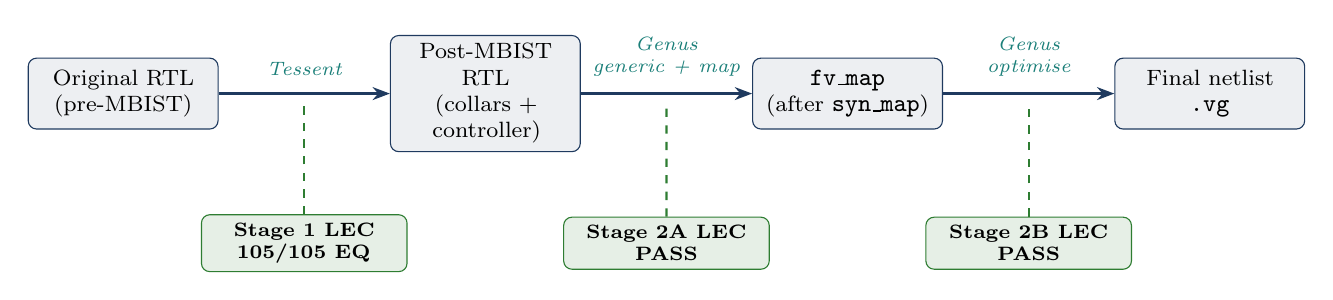
\begin{tikzpicture}
  \node[blk, text width=22mm] (rtl) at (0,0) {Original RTL\\(pre-MBIST)};
  \node[blk, text width=22mm] (mb)  at (4.6,0) {Post-MBIST RTL\\(collars + controller)};
  \node[blk, text width=22mm] (map) at (9.2,0) {\code{fv\_map}\\(after \code{syn\_map})};
  \node[blk, text width=22mm] (net) at (13.8,0) {Final netlist\\\code{.vg}};
  \draw[arr] (rtl.east) -- coordinate[midway](m1) (mb.west);
  \draw[arr] (mb.east)  -- coordinate[midway](m2) (map.west);
  \draw[arr] (map.east) -- coordinate[midway](m3) (net.west);
  \node[tool, above=1mm of m1] {Tessent};
  \node[tool, above=1mm of m2] {Genus\\generic + map};
  \node[tool, above=1mm of m3] {Genus\\optimise};

  \node[chk] (s1)  at (2.3,-1.9)  {Stage 1 LEC\\105/105 EQ};
  \node[chk] (s2a) at (6.9,-1.9)  {Stage 2A LEC\\PASS};
  \node[chk] (s2b) at (11.5,-1.9) {Stage 2B LEC\\PASS};
  \draw[leaf, thick, dashed] (s1.north)  -- (m1 |- 0,-0.1);
  \draw[leaf, thick, dashed] (s2a.north) -- (m2 |- 0,-0.1);
  \draw[leaf, thick, dashed] (s2b.north) -- (m3 |- 0,-0.1);
\end{tikzpicture}
\caption{Every transformation (top row) is paired with a formal check (green boxes) that proves
the two designs on either side are equivalent.}
\label{fig:flow}
\end{figure}

\begin{center}
\small
\begin{tabular}{@{}clp{8.2cm}@{}}
\toprule
\textbf{Task} & \textbf{Tool} & \textbf{Purpose} \\ \midrule
1 & Siemens Tessent & Insert MBIST collars, controller and IJTAG network; generate and run signoff patterns \\
2 & Siemens QuestaSim & Inspect the waveform of the March test to confirm it really exercises the memories \\
3 & Cadence Conformal & \textbf{Stage 1}: prove post-MBIST RTL $\equiv$ original RTL in mission mode \\
4 & Cadence Genus & Synthesise to standard cells with clock gating; emit LEC scripts \\
5 & Cadence Conformal & \textbf{Stage 2A + 2B}: prove RTL $\equiv$ final gate netlist, in two guided steps \\ \bottomrule
\end{tabular}
\end{center}

% =====================================================================
\section{Design Under Test}

\code{counter\_system} connects two small counters to two single-port synchronous SRAMs.

\begin{center}
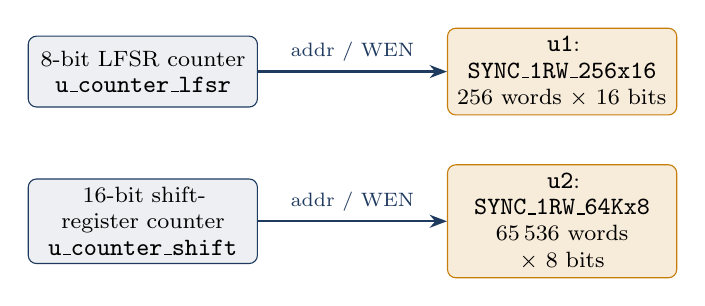
\begin{tikzpicture}[node distance=9mm]
  \node[blk] (lfsr) {8-bit LFSR counter\\\code{u\_counter\_lfsr}};
  \node[blk, below=of lfsr] (shift) {16-bit shift-register counter\\\code{u\_counter\_shift}};
  \node[blk, right=24mm of lfsr, fill=amber!15, draw=amber] (u1) {\code{u1}: \code{SYNC\_1RW\_256x16}\\256 words $\times$ 16 bits};
  \node[blk, right=24mm of shift, fill=amber!15, draw=amber] (u2) {\code{u2}: \code{SYNC\_1RW\_64Kx8}\\65\,536 words $\times$ 8 bits};
  \draw[arr] (lfsr) -- node[above, font=\scriptsize]{addr / WEN}(u1);
  \draw[arr] (shift) -- node[above, font=\scriptsize]{addr / WEN}(u2);
\end{tikzpicture}
\end{center}

\begin{itemize}
  \item In \textbf{mission mode} the counters drive the memory address and write-enable pins.
  \item In \textbf{test mode} a \emph{test collar} around each memory switches its inputs to the on-chip MBIST controller instead.
        This switch is a multiplexer controlled by a register called \code{BIST\_INPUT\_SELECT}. We will meet it again in Stage 1.
\end{itemize}

% =====================================================================
\section{Task 1: MBIST Insertion and Signoff Simulation}

\subsection{What was run}
The script \code{run\_mbist\_insertion} was executed inside Tessent Shell. Each step and its reason:

\begin{center}
\small
\begin{tabular}{@{}c p{5.6cm} p{7cm}@{}}
\toprule
\# & \textbf{Step} & \textbf{Why it is needed} \\ \midrule
1 & \code{set\_context dft -rtl -design\_id rtl1} & Tells Tessent to work on RTL (before synthesis), so the test logic is itself synthesisable. \\
2 & Read RTL, memory models (\code{.tcd\_memory}), cell library (\code{adk.tcelllib}) & Tessent needs each memory's ports, size and timing to pick a suitable March algorithm. \\
3 & \code{add\_clocks 0 clk -period 10ns} & Defines the 100\,MHz clock the controller will run on. \\
4 & \code{create\_dft\_specification} & Creates the plan: controller \code{c1}, one collar per memory, and an IJTAG network with SIBs (Scan Interface Blocks) to reach them. \\
5 & Process the specification & Actually edits the RTL: inserts collars and controller. \\
6 & Extract ICL / PDL & ICL describes the test network and PDL describes how to operate it; together they let patterns be generated automatically. \\
7 & Generate signoff patterns & \code{ICLNetwork}, \code{MemoryBist\_P1}, \code{MemoryBist\_ParallelRetentionTest\_P1}. \\
8 & Simulate with waveforms on & Gives evidence that the inserted hardware really works. \\ \bottomrule
\end{tabular}
\end{center}

\begin{whybox}[Why three pattern suites?]
Each checks a different layer. \code{ICLNetwork} proves the IJTAG access network can be
reached and shifted. \code{MemoryBist\_P1} runs the March algorithm on the memories and checks the
GO/DONE verdict. The \code{ParallelRetentionTest} tests the retention fault from Section~1
by writing, waiting, then reading back, with both memories in parallel.
\end{whybox}

\subsection{Result}
\begin{resultbox}
\centering
unscheduled 0 \quad queued 0 \quad running 0 \quad \textbf{pass 3} \quad \textbf{fail 0}\\
All three signoff pattern suites passed (100\%).
\end{resultbox}

Afterwards \code{create\_mbist\_filelist.pl} produced \code{mbist\_file\_list}: the list of all modified
RTL plus the new BIST instruments. Later steps (LEC and synthesis) read this list so that they see the
\emph{post}-MBIST design.

\begin{figure}[H]
\centering
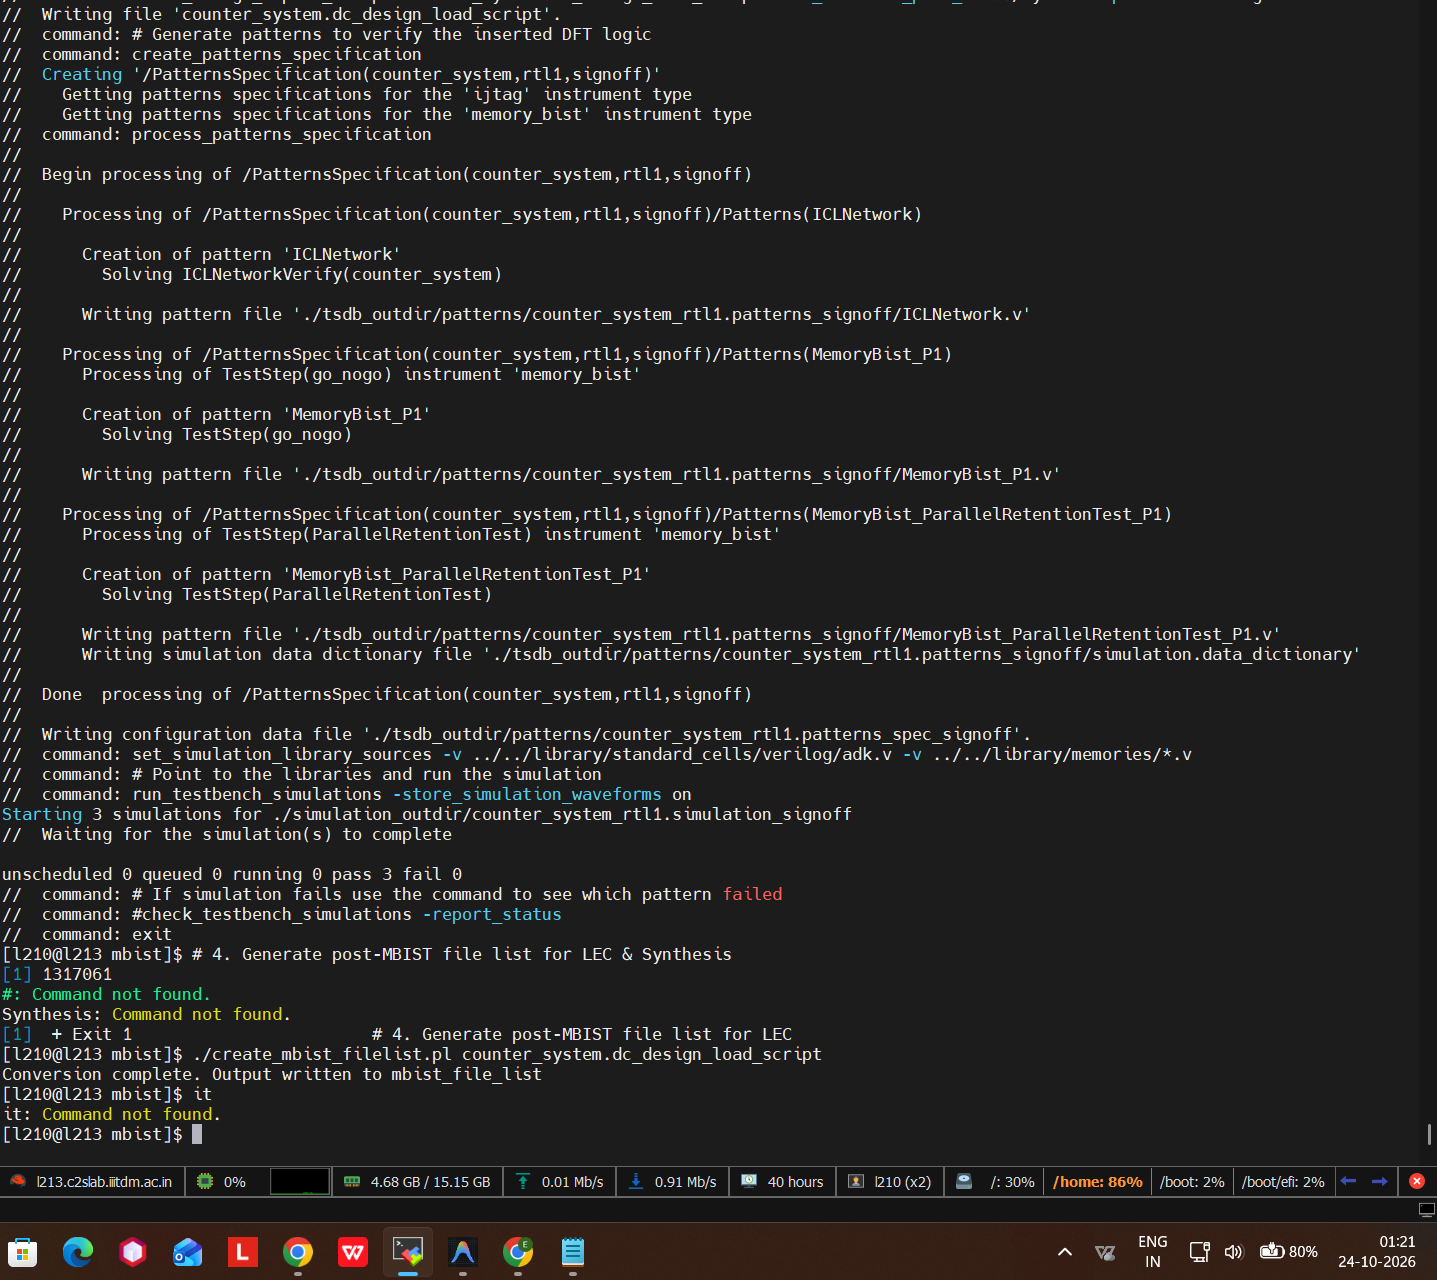
\includegraphics[width=0.93\textwidth]{images/mbist insertion.png}
\caption{Tessent log: three signoff simulations started and finished with \textbf{pass 3, fail 0}; the file list is generated at the bottom.}
\label{fig:mbist_insertion}
\end{figure}

% =====================================================================
\section{Task 2: Simulation Waveform Analysis}

Passing is good, but a waveform shows \emph{why} it passed. The primary March test was opened with:
\begin{lstlisting}[language=bash]
vsim -view simulation_outdir/counter_system_rtl1.simulation_signoff/MemoryBist_P1.simulation/vsim.wlf
\end{lstlisting}

\begin{figure}[H]
\centering
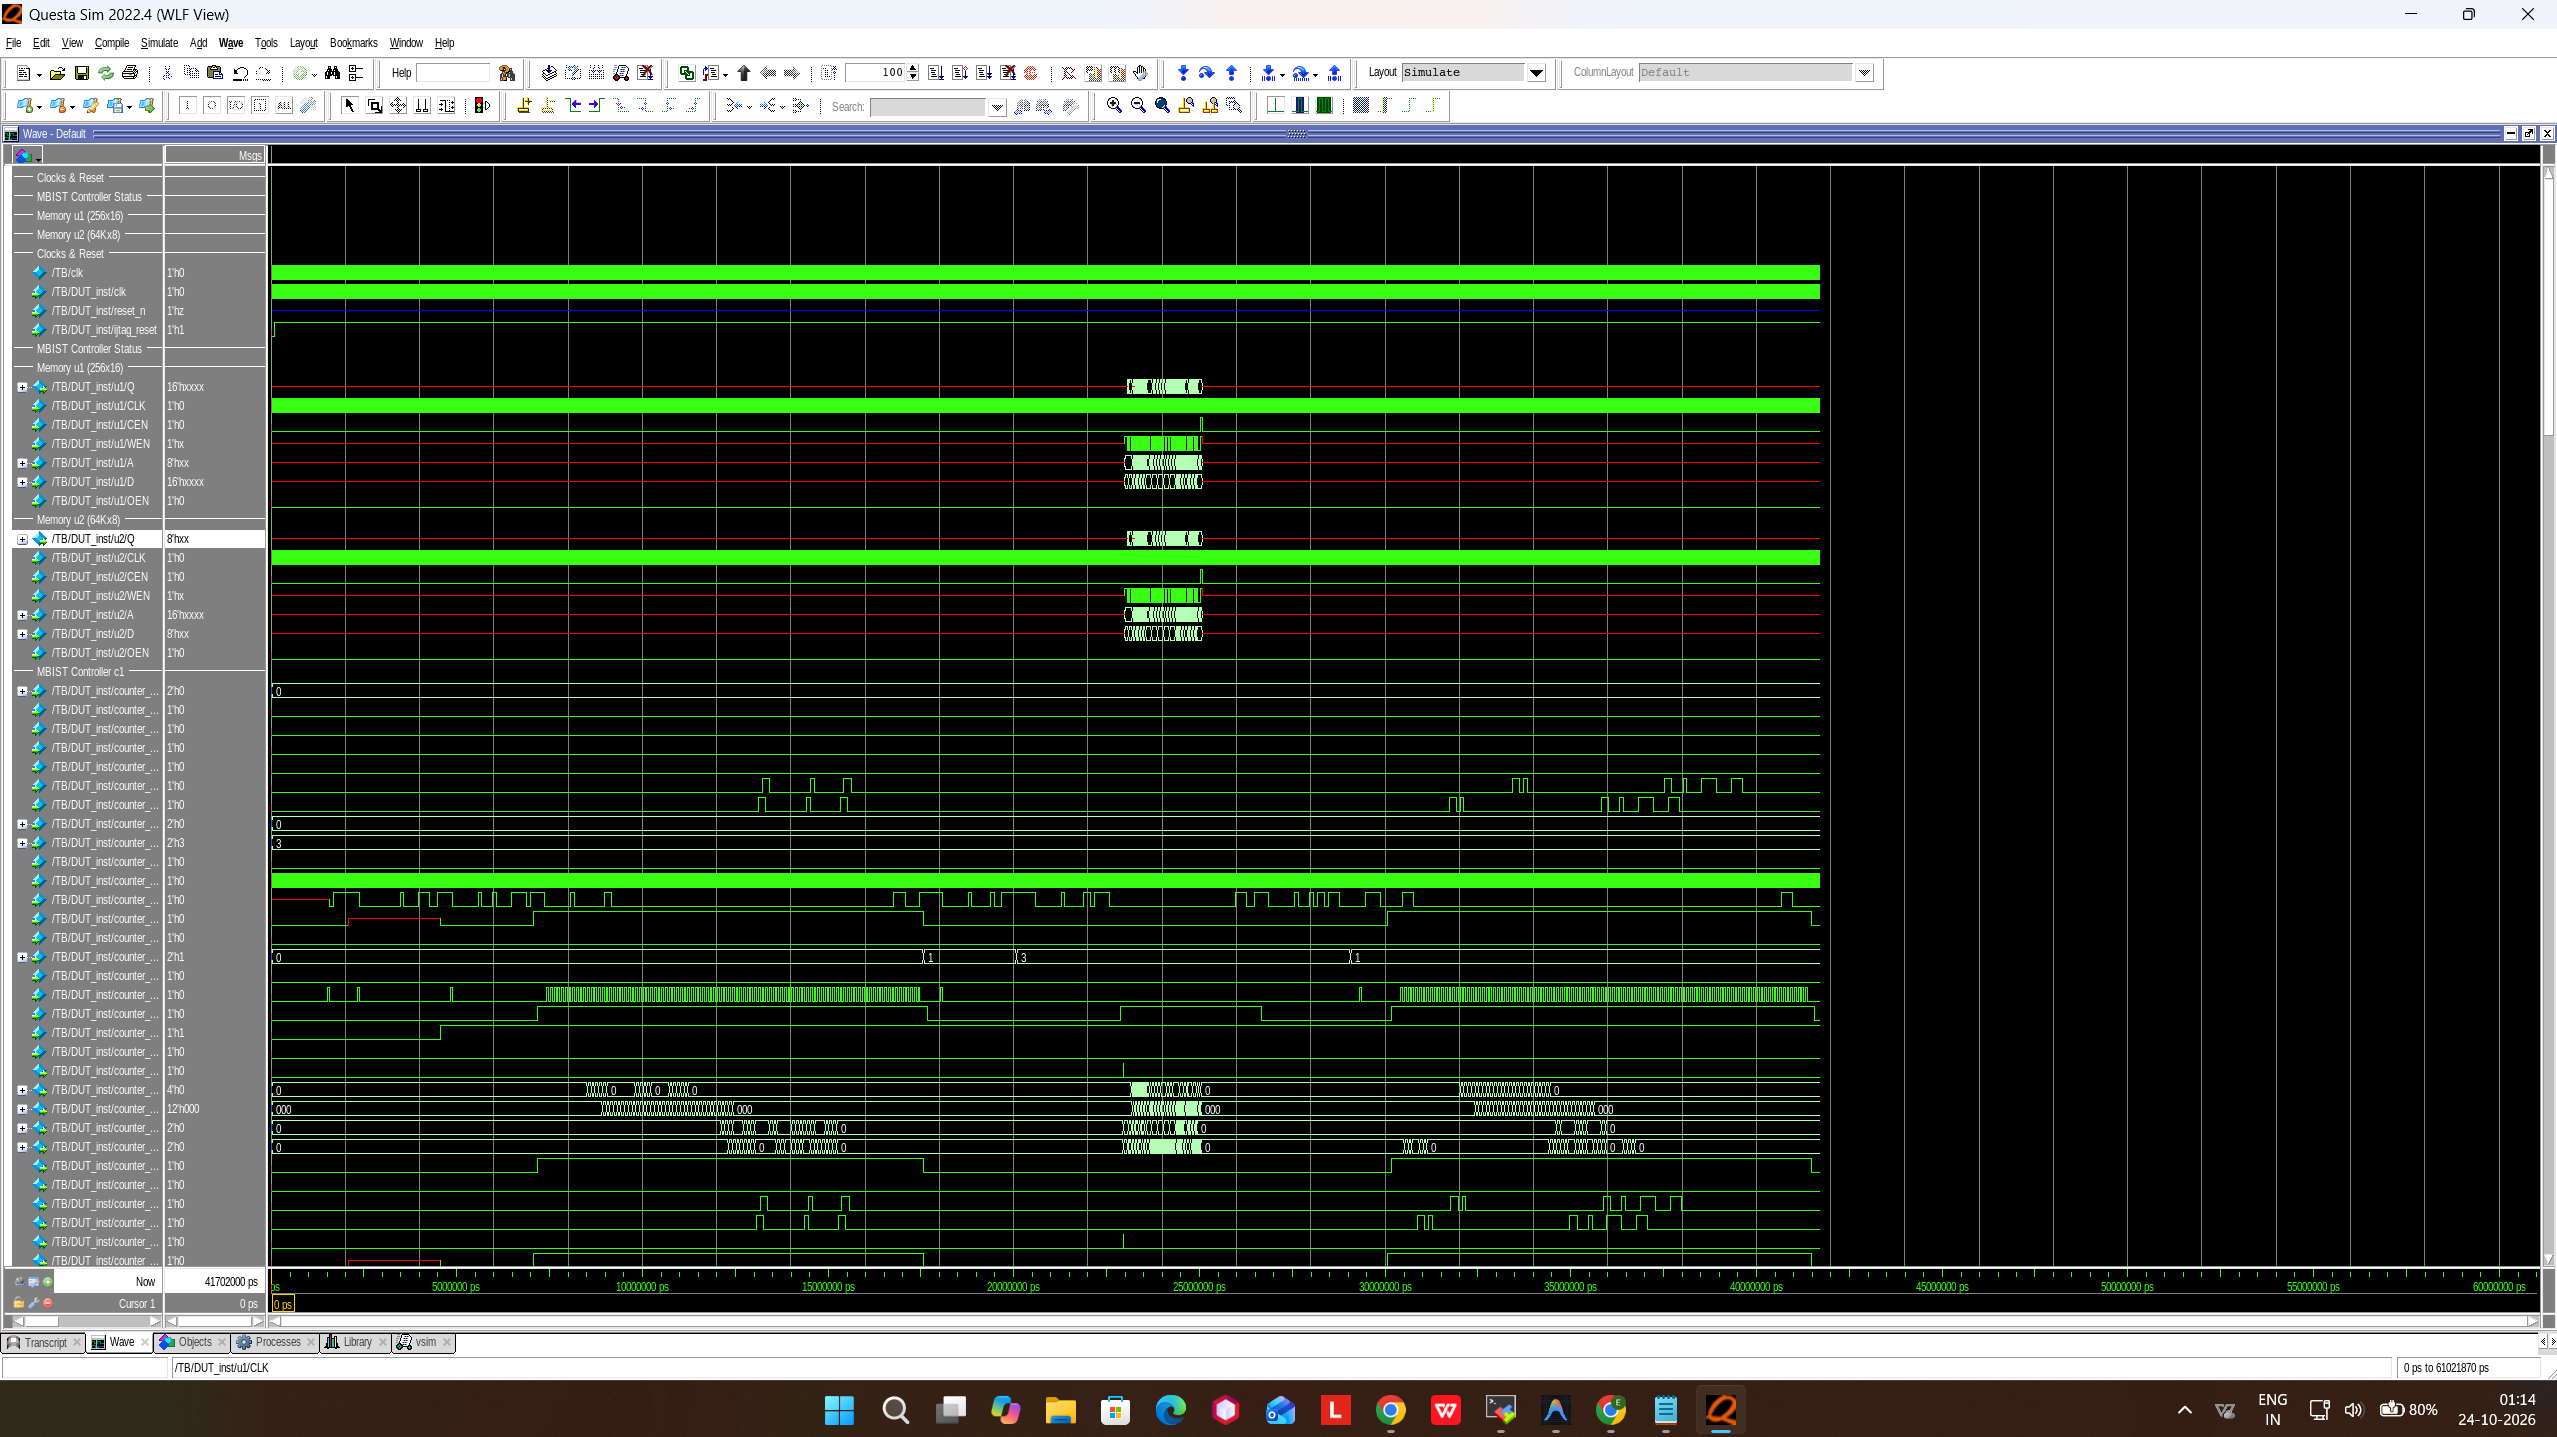
\includegraphics[width=\textwidth]{images/waveform.png}
\caption{QuestaSim waveform of \code{MemoryBist\_P1}. Bursts of activity on the memory pins are the March read/write passes.}
\label{fig:waveform}
\end{figure}

\subsection{How to read it}
\begin{center}
\small
\begin{tabular}{@{}p{3.4cm}p{11.4cm}@{}}
\toprule
\textbf{Signal(s)} & \textbf{What we see and what it means} \\ \midrule
\code{clk}, \code{reset\_n}, \code{ijtag\_reset} & 10\,ns clock (100\,MHz). The resets bring the state machines to a known starting state. \\
\code{MBISTPG\_EN}, \code{COLLAR\_EN} & The controller wakes up and the collars hand the memory pins over to it. \\
\code{CEN}, \code{WEN}, \code{A} & Chip enable and write enable pulse in bursts while the address counts through every word: a March-style \emph{write pass} followed by \emph{read-and-compare passes}, on \code{u1} and \code{u2}. \\
\code{MBISTPG\_DONE} & Goes high when the algorithm has finished all of its steps. \\
\code{MBISTPG\_GO} & Stays high: every value read back matched what was expected, i.e.\ \textbf{no memory fault detected}. \\ \bottomrule
\end{tabular}
\end{center}

\begin{keybox}[What is a March test?]
A March test sweeps the address space up and/or down, doing a few reads and writes at each address, for example
$\Uparrow(w0);\ \Uparrow(r0,w1);\ \Uparrow(r1,w0);\ \Downarrow(r0,w1);\ \Downarrow(r1,w0);\ \Updownarrow(r0)$ (this is March~C$-$).
Mixing up-sweeps and down-sweeps is what exposes coupling and address-decoder faults that a simple
``write everything, read everything'' test would miss. The burst-and-gap shape in Figure~\ref{fig:waveform} is this sweep structure.
\end{keybox}

% =====================================================================
\section{Task 3: Stage 1 Formal Verification (Original RTL vs.\ Post-MBIST RTL)}

\subsection{Objective}
MBIST adds multiplexers in front of the memories. If we made a mistake, the chip could behave differently
in normal operation even though the self-test passes. Stage 1 proves it does not.

\begin{whybox}[Why do we need pin constraints?]
The two designs are \emph{not} identical: the post-MBIST design has an extra controller, IJTAG pins and
collar multiplexers. We want to prove something narrower and more useful:
\textbf{when the chip is in mission mode, the two designs are equivalent.}
To say ``mission mode'' to the tool, we pin every test-related control to its inactive value.
\end{whybox}

\subsection{The constraints in \code{mbist.do}, line by line}
\begin{lstlisting}[language=LECTcl, caption={Stage 1 constraints}]
// Test-mode controls held inactive in BOTH designs
add pin constraints 0 scan_enable -both
add pin constraints 0 scan_mode   -both
add pin constraints 0 ijtag_reset -revised

// The IJTAG serial-out has no counterpart in the original design
add ignored outputs ijtag_so -revised

// Force the collar multiplexers to "functional" (0)
add primary input u1_interface_inst/BIST_INPUT_SELECT_reg/Q -pin -revised
add primary input u2_interface_inst/BIST_INPUT_SELECT_reg/Q -pin -revised
add pin constraints 0 u1_interface_inst/BIST_INPUT_SELECT_reg/Q -revised
add pin constraints 0 u2_interface_inst/BIST_INPUT_SELECT_reg/Q -revised
\end{lstlisting}

\begin{center}
\small
\begin{tabular}{@{}p{5.2cm}p{9.6cm}@{}}
\toprule
\textbf{Command} & \textbf{Reason} \\ \midrule
\code{pin constraints 0 scan\_enable/scan\_mode -both} & Scan shifting is a test feature. Pinning it to 0 in both designs stops the tool from exploring scan behaviour. \\
\code{pin constraints 0 ijtag\_reset -revised} & Keeps the IJTAG network idle; only the revised design has this pin. \\
\code{ignored outputs ijtag\_so -revised} & \code{ijtag\_so} exists only in the revised design, so there is nothing to compare it against. \\
\code{add primary input \ldots/BIST\_INPUT\_SELECT\_reg/Q -pin} & \code{BIST\_INPUT\_SELECT\_reg} is a flip-flop \emph{inside} the design, so it cannot be constrained directly. This command re-labels its output as a pseudo primary input so that a constraint can be applied. \\
\code{pin constraints 0 \ldots/Q} & Sets that signal to 0, so the collar multiplexer permanently selects the \emph{functional} path (counters $\to$ memory). \\ \bottomrule
\end{tabular}
\end{center}

\subsection{Result, and how to read the log}
\begin{resultbox}
\textbf{105 compare points equivalent, 0 non-equivalent, 0 aborted.}\\
51 primary outputs\; +\; 52 flip-flops\; +\; 2 memory black boxes\; =\; 105.
\end{resultbox}

The tool log (Figure~\ref{fig:stage1_lec}) gives a nice sanity check that nothing was hidden by the constraints:

\begin{center}
\small
\begin{tabular}{@{}lcccc@{}}
\toprule
 & \textbf{Golden} & \textbf{Revised} & \textbf{Mapped} & \textbf{Left over in Revised} \\ \midrule
Key points & 139 & 424 & 139 & 285 \\ \bottomrule
\end{tabular}
\end{center}

The revised design has $424-139 = 285$ extra key points. The log classifies them as
\textbf{6 ``extra''} (the new IJTAG inputs such as \code{ijtag\_tck}, which have no counterpart in the original) and
\textbf{279 ``unreachable''} (264 DFFs + 15 latches: the MBIST controller and collars, which cannot affect any output while MBIST is
held off). Every one of the original 139 key points was matched one-to-one, and all
compared equal. In other words: \emph{all the extra hardware is test-only, and the original logic is untouched.}

\begin{figure}[H]
\centering
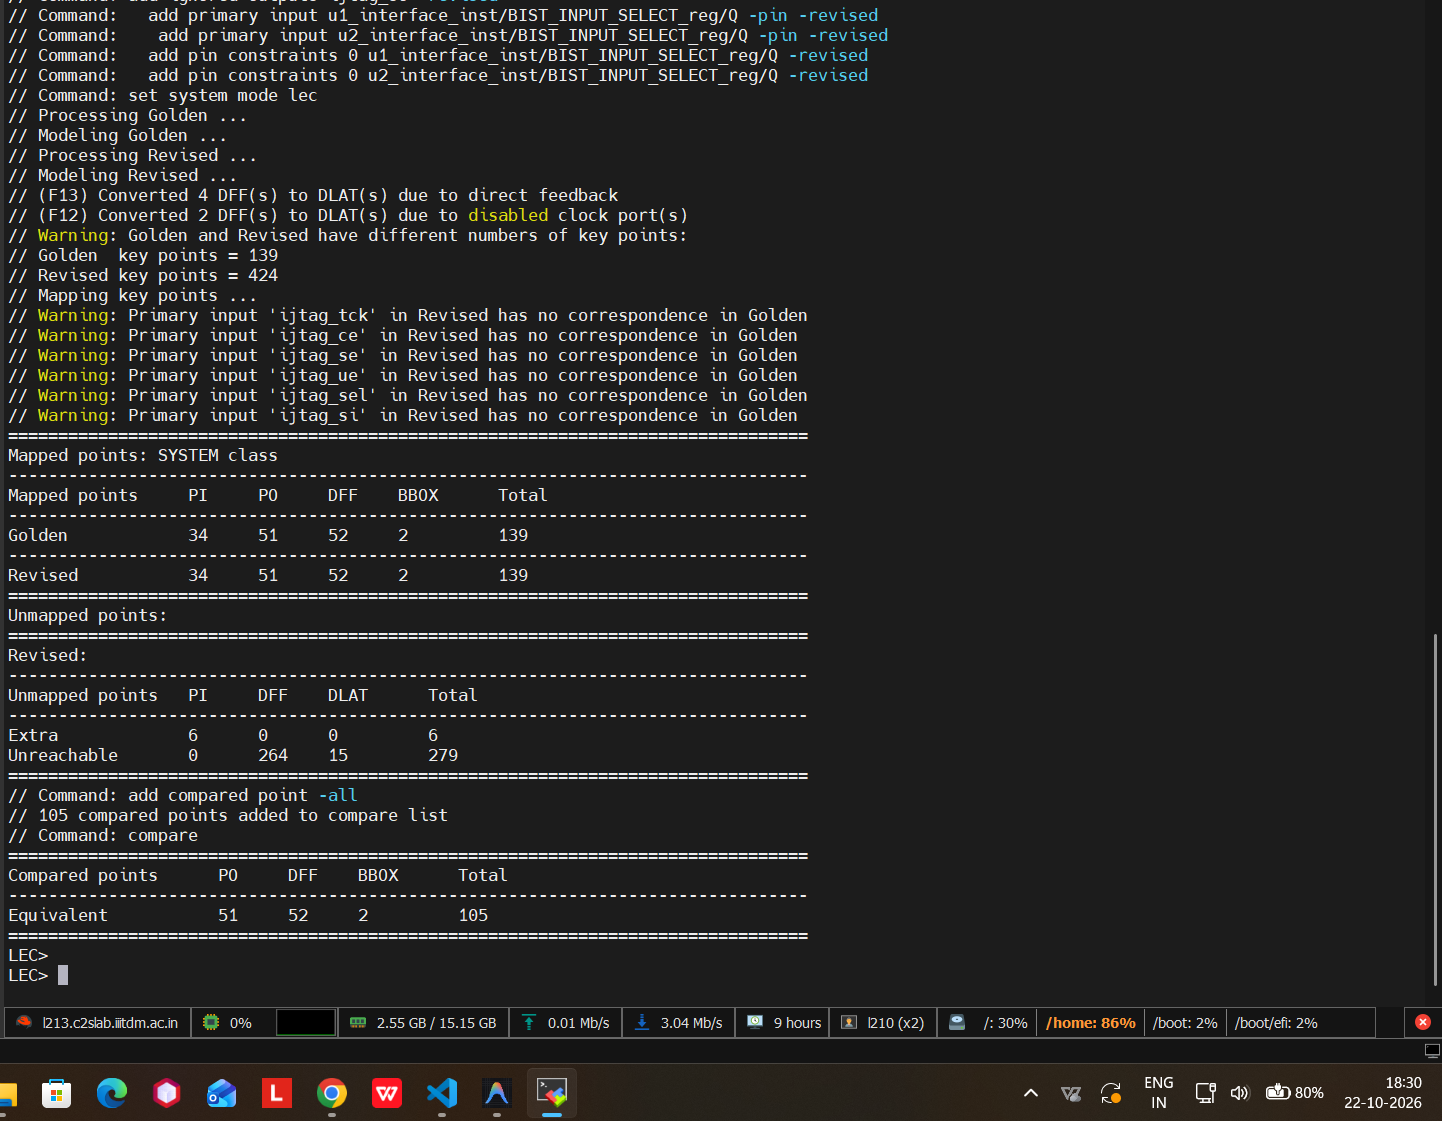
\includegraphics[width=0.9\textwidth]{images/stage1_lec_pass.png}
\caption{Stage 1 LEC log: mapped-points table and the final \texttt{Equivalent 105} line.}
\label{fig:stage1_lec}
\end{figure}

% =====================================================================
\section{Task 4: Logic Synthesis with Clock Gating (Cadence Genus)}

\subsection{What synthesis does}
Synthesis turns RTL (behavioural Verilog) into a \emph{gate-level netlist} built from the real standard cells in \code{adk.lib}.
Along the way, the tool is free to restructure the logic to save area, power and delay.
That freedom is exactly why a formal check is needed afterwards.

\begin{lstlisting}[language=LECTcl, caption={Genus \texttt{run.tcl}, annotated}]
source setup.tcl
set design_name counter_system

// Load the post-MBIST RTL and the memories (as black-box wrappers)
source ../mbist/${design_name}.dc_design_load_script
read_hdl ../../library/memories/SYNC_1RW_256x16.v_interface \
         ../../library/memories/SYNC_1RW_64Kx8.v_interface
elaborate
current_design ${design_name}
source ../constraints/constraints.sdc
source ./mbist_postelab.tcl

// Save power by gating clocks of registers that often hold their value
set_db lp_insert_clock_gating true

syn_generic                 // technology-independent optimisation
syn_map                     // map to library cells  -> "fv_map" snapshot
write_do_lec -golden rtl -revised fv_map -logfile rtl2map.log > ../lec/rtl2fvmap1.tcl   // Stage 2A script

syn_opt                     // incremental optimisation (timing / area / power)
write_sdc $design_name > ${design_name}.merged_sdc
write_netlist > $design_name.vg
write_do_lec -golden fv_map -revised $design_name.vg -logfile fvmap2final.log > ../lec/fvmap2final1.tcl   // Stage 2B script
\end{lstlisting}

\begin{whybox}[Why these particular lines?]
\begin{itemize}
  \item \textbf{Memories as black boxes.} SRAM macros are not made of standard cells and are not synthesised. They are supplied as empty
        interface wrappers (Genus reports \code{VLD-18/VRD-14: logic abstract} for \code{SYNC\_SRAM\_256x16} and \code{64Kx8}), and LEC
        later compares them by their pins, which is why \emph{BBOX} appears among the compare points.
  \item \textbf{\code{lp\_insert\_clock\_gating true}.} Instead of using a multiplexer to ``recirculate'' a register's old value when it is not being written,
        the tool stops the clock to the register. This saves dynamic power. It also changes the clocking structure, which will matter in Section~\ref{sec:two-stage}.
  \item \textbf{\code{write\_do\_lec} twice, at two different moments.} The script is dumped \emph{between} \code{syn\_map} and \code{syn\_opt} as well as at the end.
        This is what creates the intermediate design \code{fv\_map} on which the two-stage check depends.
\end{itemize}
\end{whybox}

\begin{figure}[H]
\centering
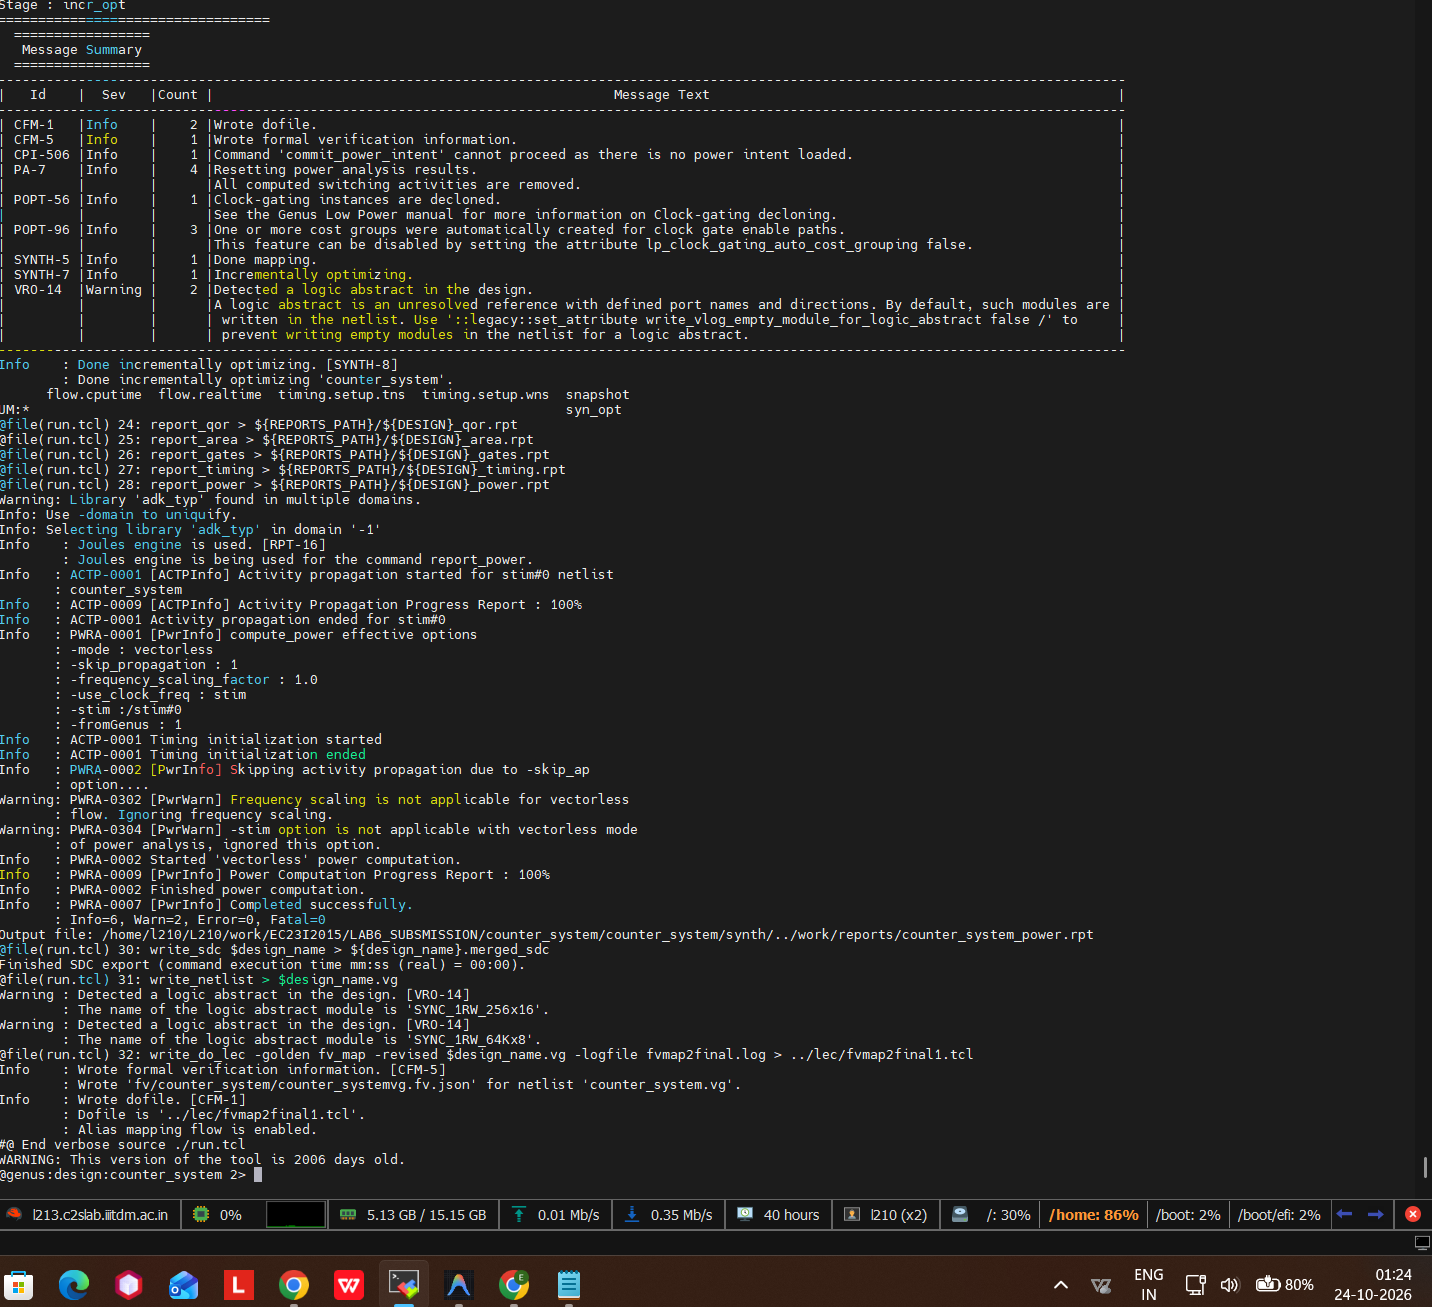
\includegraphics[width=0.9\textwidth]{images/genus_run.png}
\caption{Genus run. The message summary lists \code{POPT-56} (clock-gating instances declared), power/area/timing reports being written, and the formal-verification files (\code{.fv.json} and \code{fvmap2final1.tcl}) being produced.}
\label{fig:genus_run}
\end{figure}

\textbf{Outputs:} \code{counter\_system.vg} (gate netlist), \code{counter\_system.merged\_sdc} (constraints), reports for area, gates, timing, power and QoR, and the two LEC dofiles.

\subsection{Cost of MBIST: pre-MBIST vs post-MBIST synthesis}
\label{sec:ppa}

To measure what the test hardware costs, the original \code{counter\_system} RTL (no MBIST) was synthesised as a \emph{baseline}
with a separate script, \code{synth\_pre/run\_pre.tcl}. It differs from \code{run.tcl} only where MBIST is involved: it reads the original RTL
instead of the Tessent-modified files, and it skips \code{mbist\_postelab.tcl} and \code{write\_do\_lec}. Everything else is identical for a fair
comparison: same libraries, same \code{constraints.sdc} (10\,ns clock), clock gating on, and the same \code{syn\_generic}/\code{syn\_map}/\code{syn\_opt} flow.
Its outputs go to separate folders, so the post-MBIST results above are untouched.

\begin{table}[H]
\centering
\begin{tabular}{@{}lrrr@{}}
\toprule
\textbf{Metric} & \textbf{Pre-MBIST} & \textbf{Post-MBIST} & \textbf{Change} \\
\midrule
Cell area                 & 334.212   & 3578.971  & $+3244.759$ ($10.7\times$) \\
Instance count            & 119       & 1745      & $+1626$ ($14.7\times$) \\
Worst setup slack (ps)    & 2405      & 2128      & $-277$ \\
Total power (mW)          & 0.258     & 3.136     & $+2.878$ ($12.2\times$) \\
\quad clock power (mW)    & 0.153     & 2.438     & $+2.285$ \\
\quad register power (mW) & 0.039     & 0.173     & $+0.133$ \\
\quad logic power (mW)    & 0.065     & 0.523     & $+0.458$ \\
\bottomrule
\end{tabular}
\caption{Pre-MBIST vs post-MBIST synthesis results from the Genus reports (\code{counter\_system\_area/gates/timing/power.rpt}).}
\label{tab:ppa}
\end{table}

\textbf{Reading the table.}
\begin{itemize}
  \item \textbf{Area and instances.} The post-MBIST design is about ten times larger. Of its area, the Tessent controller is 1859 (about 52\%), the two memory interfaces 545 and 391, the access port (BAP) 311 and the two SIBs 107 and 28. The remaining $\approx$338 is the original counter logic, which matches the 334 of the baseline: \emph{the whole increase is test hardware.} The SRAM macros are black boxes and are not counted in either run.
  \item \textbf{Timing.} Both designs meet timing with a large margin. The two slacks are from different kinds of path: the post-MBIST worst path is a clock-gating setup check inside the controller, so the $-277$\,ps is not a like-for-like slowdown.
  \item \textbf{Power.} Clock power dominates after MBIST (77.7\% of the total, against 59.3\% before), because the controller and interfaces add many registers and clock-gating cells. The figures are vectorless switching power only; the library reports zero leakage and internal power in both runs.
\end{itemize}

% =====================================================================
\section{Task 5: Stage 2 Formal Verification -- Why Two Stages?}
\label{sec:two-stage}

This section is the heart of the lab. We follow it as a story: \emph{what we tried, what broke, why it broke, and what fixes it.}

\subsection{Attempt 1: compare post-MBIST RTL directly with the final netlist}

The obvious check is a single comparison: golden = post-MBIST RTL, revised = \code{counter\_system.vg}.

\begin{probbox}[Observed result]
\begin{itemize}
  \item Primary outputs: all matched.
  \item Memory black boxes: both matched.
  \item \textbf{65 flip-flops: NON-EQUIVALENT.}
\end{itemize}
\end{probbox}

The outputs match, so the chip \emph{behaves} the same. Yet the tool reports failures. So are the 65 flops genuinely broken?
No: the failure is in the \emph{comparison method}, not in the design. To see why, we first need to know how LEC works.

\subsection{Background: how LEC compares two designs}

\begin{keybox}[LEC in one paragraph]
LEC cuts each design at its registers, memories and ports. Those cut points are called \textbf{key points}. It then \textbf{maps} each key point in the golden design to its
partner in the revised design (mostly by matching names and structure). Finally it proves that the combinational logic
feeding every mapped pair is identical. If every pair matches, the two sequential machines are equivalent.
\end{keybox}

This method has one important assumption: \textbf{every register on one side has a partner register on the other side.}
Anything that breaks this one-to-one assumption makes the tool either fail to map a register or fail to prove it.
Synthesis breaks it in two ways.

\subsection{Why synthesis breaks the one-to-one assumption}

\subsubsection{Cause 1 -- Sequential register merging}
The Tessent MBIST controller contains several control registers (for example \code{EXECUTE\_ADD\_Y1\_CMD\_REG0\_reg}
and \code{EXECUTE\_LOOP\_CMD\_REG1\_reg}) \sloppy that have the \emph{same clock, same reset and same next-state logic}. They always hold the same value, so they are redundant. To save area, Genus keeps one and deletes the others, reconnecting all their fan-out to the survivor.

\begin{figure}[H]
\centering
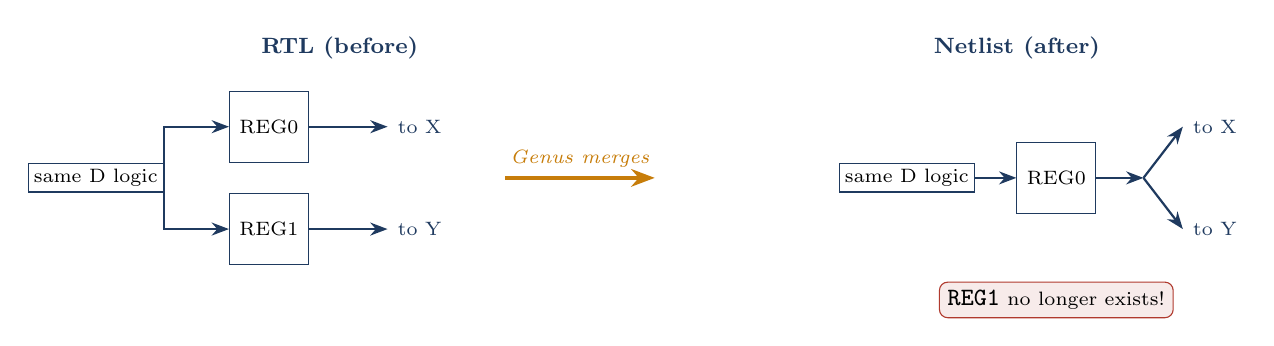
\begin{tikzpicture}[node distance=8mm]
  % before
  \node[font=\footnotesize\bfseries, text=navy] at (1.9,2.5) {RTL (before)};
  \node[ff] (a) at (1,1.5) {REG0};
  \node[ff] (b) at (1,0.2) {REG1};
  \node[gate] (d) at (-1.2,0.85) {same D logic};
  \draw[arr] (d.east) |- (a.west);
  \draw[arr] (d.east) |- (b.west);
  \draw[arr] (a.east) -- ++(1,0) node[right, font=\scriptsize]{to X};
  \draw[arr] (b.east) -- ++(1,0) node[right, font=\scriptsize]{to Y};

  \draw[-{Stealth[length=3mm]}, very thick, amber] (4.0,0.85) -- node[above, font=\scriptsize\itshape, text=amber]{Genus merges}(5.9,0.85);

  % after
  \begin{scope}[xshift=2.2cm]
  \node[font=\footnotesize\bfseries, text=navy] at (8.3,2.5) {Netlist (after)};
  \node[ff] (m) at (8.8,0.85) {REG0};
  \node[gate] (d2) at (6.9,0.85) {same D logic};
  \draw[arr] (d2.east) -- (m.west);
  \draw[arr] (m.east) -- ++(0.6,0) coordinate(j);
  \draw[arr] (j) -- ++(0.5,0.65) node[right, font=\scriptsize]{to X};
  \draw[arr] (j) -- ++(0.5,-0.65) node[right, font=\scriptsize]{to Y};
  \node[bad, font=\scriptsize] at (8.8,-0.7) {\code{REG1} no longer exists!};
  \end{scope}
\end{tikzpicture}
\caption{After merging, the golden design has a register (\code{REG1}) with no partner in the revised design.}
\end{figure}

A name-based mapper looks for \code{EXECUTE\_LOOP\_CMD\_REG1\_reg} in the netlist, finds nothing, and cannot compare it. The merge is \emph{correct}, but the tool cannot know that.

\subsubsection{Cause 2 -- Clock-gating changes the clocking structure}
With \code{lp\_insert\_clock\_gating}, Genus (message \code{POPT-56}) replaces enable logic by an integrated clock-gating cell.

\begin{figure}[H]
\centering
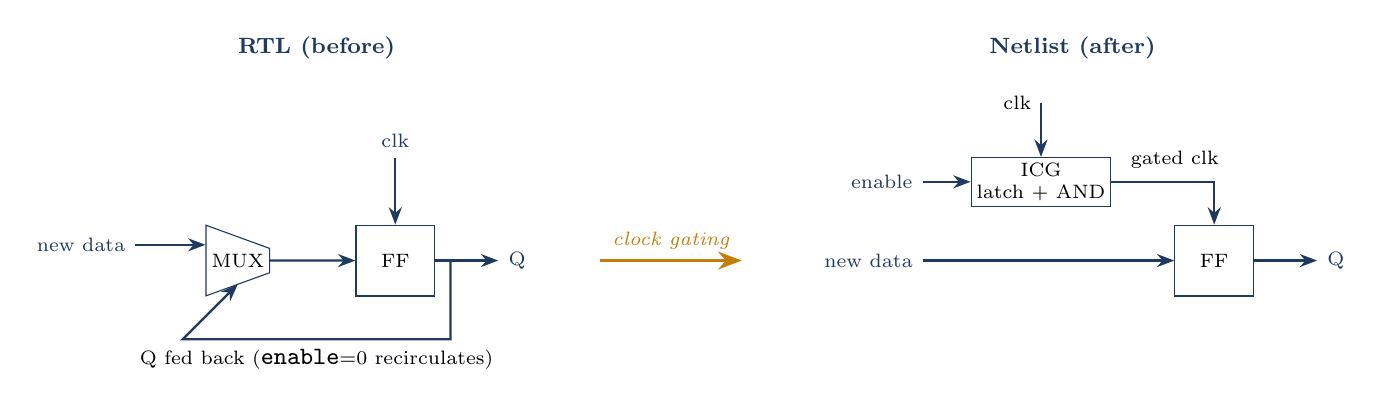
\begin{tikzpicture}
  % before
  \node[font=\footnotesize\bfseries, text=navy] at (1.6,3.7) {RTL (before)};
  \node[gate, trapezium, trapezium angle=70, shape border rotate=270, minimum height=8mm] (mux) at (0.6,1) {\scriptsize MUX};
  \node[ff] (f1) at (2.6,1) {FF};
  \draw[arr] (-0.7,1.2) node[left, font=\scriptsize]{new data} -- (mux.west |- 0,1.2);
  \draw[arr] (mux.east) -- (f1.west);
  \draw[arr] (f1.east) -- ++(0.8,0) node[right, font=\scriptsize]{Q};
  \draw[arr] (3.3,1) -- ++(0,-1.0) -- ++(-3.4,0) -- (mux.south |- 0,0.7);
  \node[font=\scriptsize] at (1.6,-0.25) {Q fed back (\code{enable}=0 recirculates)};
  \draw[arr] (2.6,2.3) node[above, font=\scriptsize]{clk} -- (f1.north);

  \draw[-{Stealth[length=3mm]}, very thick, amber] (5.2,1) -- node[above, font=\scriptsize\itshape, text=amber]{clock gating}(7.0,1);

  % after
  \begin{scope}[xshift=1.6cm]
  \node[font=\footnotesize\bfseries, text=navy] at (9.6,3.7) {Netlist (after)};
  \node[gate, align=center] (icg) at (9.2,2.0) {ICG\\\scriptsize latch + AND};
  \node[ff] (f2) at (11.4,1) {FF};
  \draw[arr] (9.2,3.0) -- (icg.north);
  \node[font=\scriptsize, left] at (9.2,3.0) {clk};
  \draw[arr] (7.7,2.0) node[left, font=\scriptsize]{enable} -- (icg.west);
  \draw[arr] (icg.east) -| (f2.north);
  \node[font=\scriptsize, above] at (10.9,2.05) {gated clk};
  \draw[arr] (7.7,1.0) node[left, font=\scriptsize]{new data} -- (f2.west);
  \draw[arr] (f2.east) -- ++(0.8,0) node[right, font=\scriptsize]{Q};
  \end{scope}
\end{tikzpicture}
\caption{Same function, different structure: the multiplexer and its feedback loop disappear and the flop's clock is gated by \code{enable}.}
\end{figure}

The register still exists, but its clock, data cone and feedback path look different, so a naive mapping and proof can no longer line up the two designs.

\begin{probbox}[Putting the two causes together]
Genus made two correct but structurally invasive optimisations. LEC, comparing registers one-to-one,
could not map the removed or restructured ones. Hence \textbf{65 ``non-equivalent'' flip-flops, even though the design is functionally right.}
The only way forward is to \emph{tell LEC what Genus did}.
\end{probbox}

\subsection{The solution: tell LEC what happened, in smaller pieces}

Genus records the sequential changes it makes in a \textbf{formal-verification guidance database}
(\code{counter\_systemvg.fv.json}; Genus message \code{CFM-5}: ``wrote formal verification information''). The \code{write\_do\_lec} command turns this into
a ready-to-run LEC script that loads the guidance. Two ideas make it robust:

\begin{enumerate}
  \item \textbf{Use the guidance.} Where Genus says ``REG1 was merged into REG0'', LEC is told the same, so the missing partner is no longer a mystery.
  \item \textbf{Split the journey into two shorter hops with an intermediate design.}
        Rather than prove one huge transformation, we save a snapshot after \code{syn\_map} (\code{fv\_map}) and prove two smaller ones.
\end{enumerate}

\begin{figure}[H]
\centering
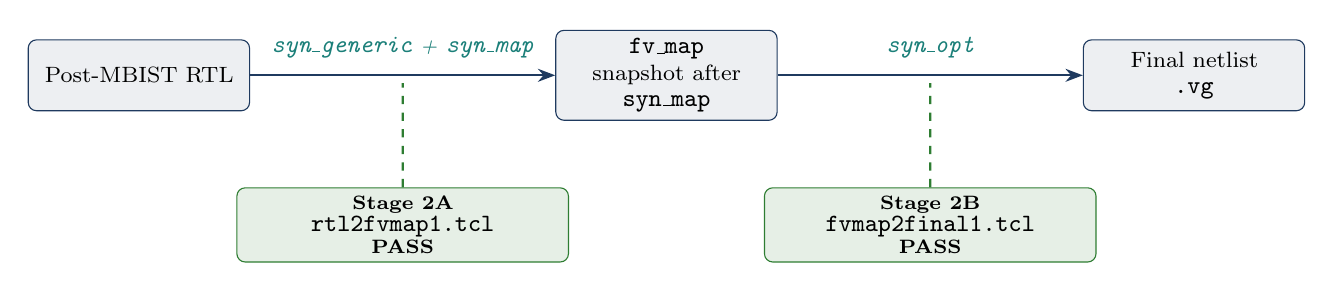
\begin{tikzpicture}
  \node[blk, text width=26mm] (r) at (1.5,0) {Post-MBIST RTL};
  \node[blk, text width=26mm] (f) at (8.2,0) {\code{fv\_map}\\snapshot after\\\code{syn\_map}};
  \node[blk, text width=26mm] (n) at (14.9,0) {Final netlist\\\code{.vg}};
  \draw[arr] (r.east) -- coordinate[midway](m1) (f.west);
  \draw[arr] (f.east) -- coordinate[midway](m2) (n.west);
  \node[tool, above=1mm of m1] {\code{syn\_generic} + \code{syn\_map}};
  \node[tool, above=1mm of m2] {\code{syn\_opt}};

  \node[chk, text width=40mm] (a) at (4.85,-1.9) {Stage 2A\\\code{rtl2fvmap1.tcl}\\PASS};
  \node[chk, text width=40mm] (b) at (11.55,-1.9) {Stage 2B\\\code{fvmap2final1.tcl}\\PASS};
  \draw[leaf, thick, dashed] (a.north) -- (m1 |- 0,-0.1);
  \draw[leaf, thick, dashed] (b.north) -- (m2 |- 0,-0.1);
\end{tikzpicture}
\caption{The two-stage LEC flow. Each hop is proven separately, so equivalence of RTL and final netlist follows by transitivity.}
\label{fig:twostage}
\end{figure}

\begin{keybox}[Why does splitting help?]
\begin{itemize}
  \item \textbf{Smaller proof obligations.} Each hop contains fewer transformations, so fewer registers lose their partner and the solver has an easier job.
  \item \textbf{Each stage gets its own guidance.} The recorded merges/gating decisions are matched to the step that produced them, so LEC applies them where they belong.
  \item \textbf{Failures are localised.} If a stage fails, we immediately know which synthesis step to investigate. The one-step approach only says ``something between RTL and netlist is wrong''.
  \item \textbf{Transitivity gives the full guarantee.}
        If RTL $\equiv$ \code{fv\_map} and \code{fv\_map} $\equiv$ netlist, then RTL $\equiv$ netlist.
\end{itemize}
\end{keybox}

\subsection{Stage 2A -- Post-MBIST RTL $\rightarrow$ \code{fv\_map} \; (\code{rtl2fvmap1.tcl})}
Run with \code{lec -XL -nogui -dofile rtl2fvmap1.tcl}. The golden side is the post-MBIST RTL; the revised side is the design after \code{syn\_generic} and \code{syn\_map}.
This stage covers the first, largest restructuring (technology-independent optimisation and mapping to gates).

\begin{figure}[H]
\centering
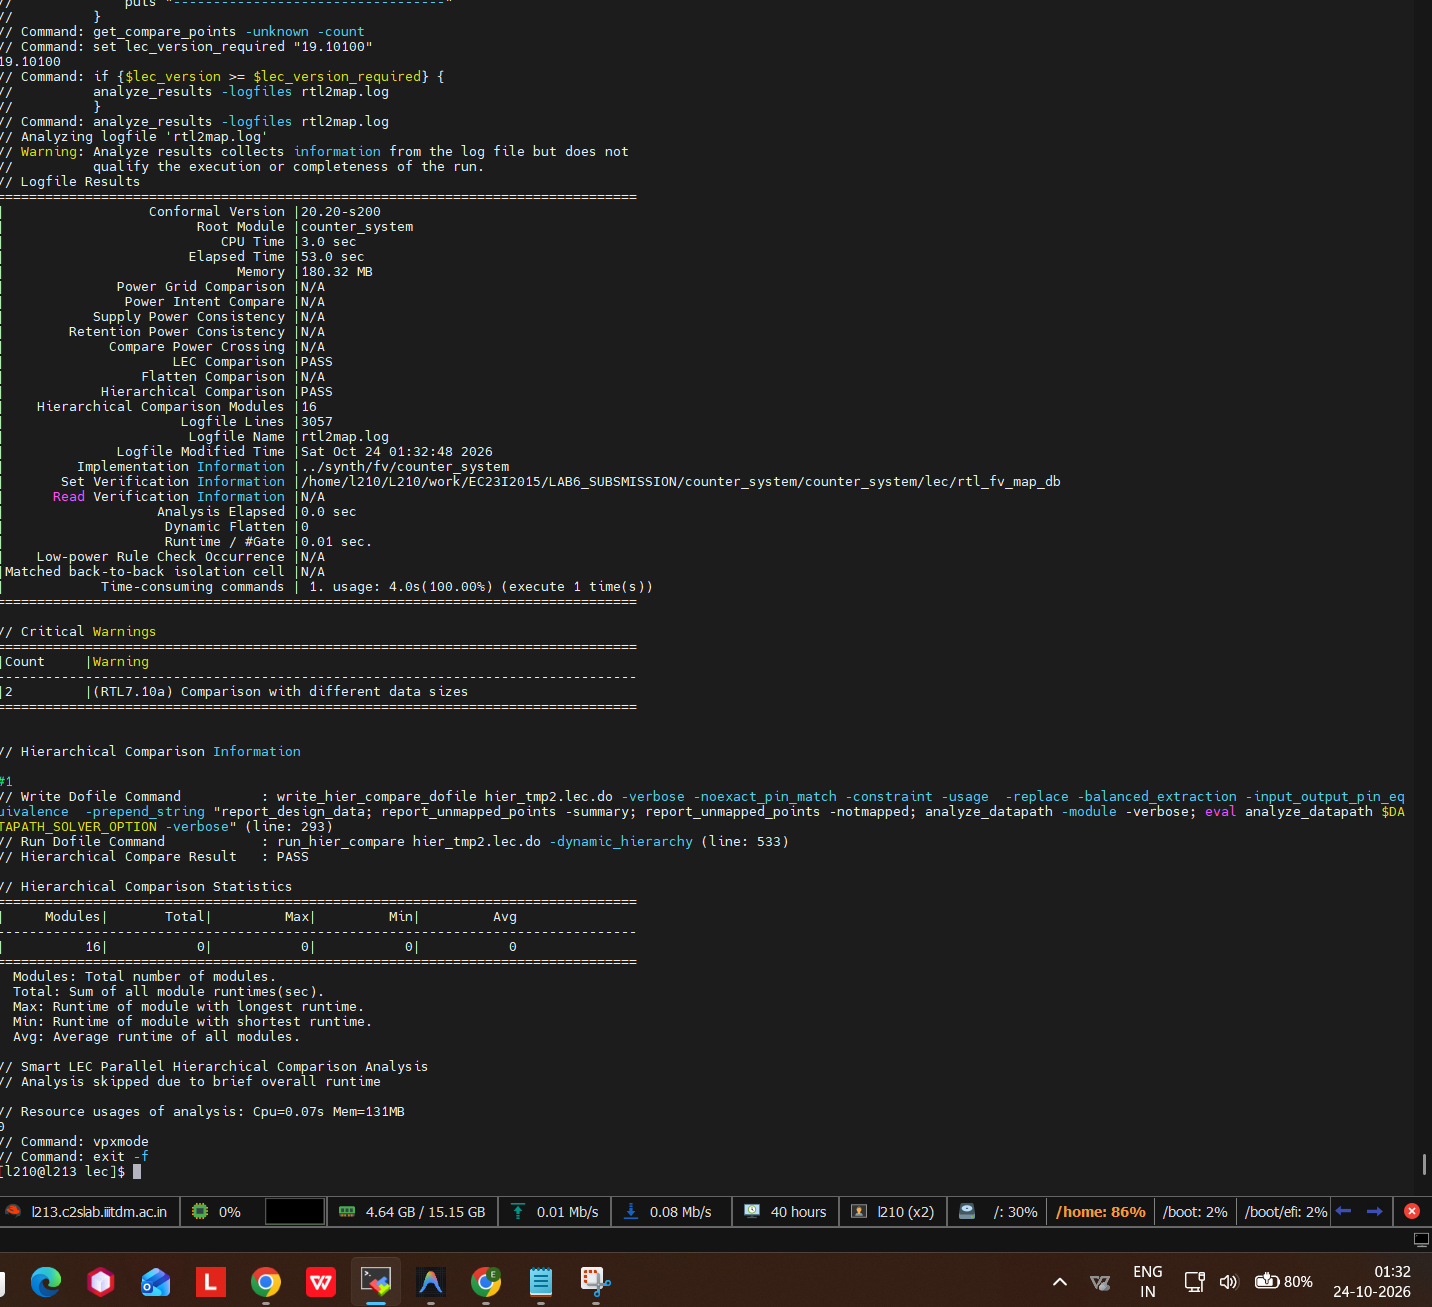
\includegraphics[width=0.9\textwidth]{images/2A_First_stage lec.png}
\caption{Stage 2A log: \code{LEC Comparison PASS} and \code{Hierarchical Comparison PASS} over 16 modules (Conformal 20.20-s200, about 3\,s CPU).}
\label{fig:stage2a}
\end{figure}

\begin{resultbox}[Stage 2A result]
\textbf{PASS.} The hierarchical comparison covered 16 modules with 0 failing. The log also lists two ``Comparison with different data sizes'' warnings; no compare point failed.
\end{resultbox}

\subsection{Stage 2B -- \code{fv\_map} $\rightarrow$ final netlist \; (\code{fvmap2final1.tcl})}
Run with \code{lec -XL -nogui -dofile fvmap2final1.tcl}. The golden side is now \code{fv\_map} (the intermediate design), the revised side is \code{counter\_system.vg}. This hop covers \code{syn\_opt}, where
Genus's clock-gating message (\code{POPT-56}) is reported, and it uses the guidance file \code{counter\_systemvg.fv.json}.

\begin{figure}[H]
\centering
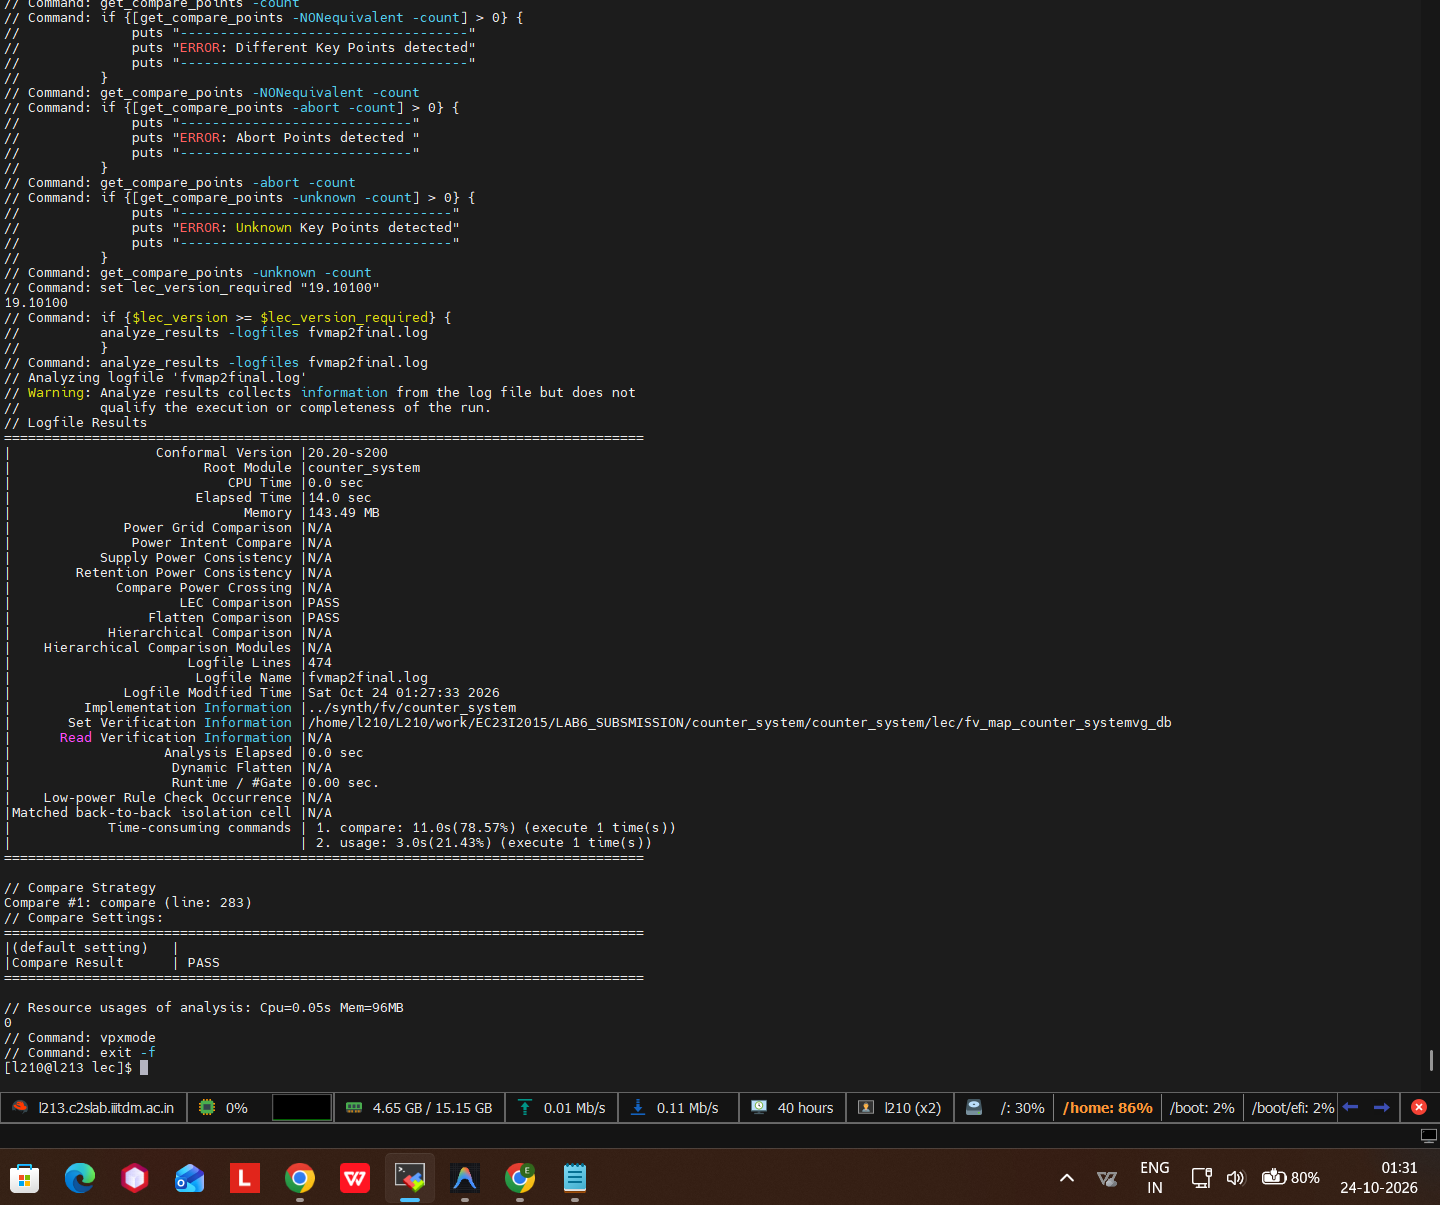
\includegraphics[width=0.9\textwidth]{images/2A_second_stage_lec.png}
\caption{Stage 2B log: the script checks for non-equivalent, aborted and unknown points (all zero) and prints \code{Compare Result PASS}.}
\label{fig:stage2b}
\end{figure}

\begin{resultbox}[Stage 2B result]
\textbf{PASS.} The comparison finished with zero non-equivalent, zero abort and zero unknown points
(compare step $\approx$ 11\,s). The 65 earlier failures have disappeared, confirming that they were a limitation of the one-step method, not real functional differences.
\end{resultbox}

\subsection{Before vs.\ after at a glance}
\begin{center}
\small
\begin{tabular}{@{}p{3.8cm}p{5.3cm}p{5.3cm}@{}}
\toprule
 & \textbf{One-step (RTL vs.\ netlist)} & \textbf{Two-stage (guided)} \\ \midrule
Comparison & RTL $\leftrightarrow$ final \code{.vg} & RTL $\leftrightarrow$ \code{fv\_map} $\leftrightarrow$ \code{.vg} \\
Knowledge of Genus's merges / gating & None; relies on name matching & Loaded from Genus's guidance database \\
Outputs and memories & Match & Match \\
Flip-flops & \textcolor{brick}{\textbf{65 non-equivalent}} & \textcolor{leaf}{\textbf{All equivalent (PASS)}} \\
Debugging a failure & Hard: whole flow is suspect & Easy: one synthesis stage is suspect \\ \bottomrule
\end{tabular}
\end{center}

% =====================================================================
\section{Summary of Deliverables}

\begin{center}
\small
\begin{tabular}{@{}p{3.1cm}p{3.1cm}p{3.5cm}p{4.6cm}@{}}
\toprule
\textbf{Phase} & \textbf{Tool} & \textbf{Result} & \textbf{Artifact / log} \\ \midrule
MBIST insertion & Siemens Tessent & 3/3 patterns PASS & \code{run\_mbist\_insertion.log} \\
P1 March simulation & Siemens QuestaSim & GO\,=\,1, DONE\,=\,1 & \code{MemoryBist\_P1/vsim.wlf} \\
Stage 1 LEC & Cadence Conformal & 105/105 equivalent & \code{mbist.do}, \code{mbist\_lec.log} \\
Logic synthesis & Cadence Genus & Netlist and reports written & \code{counter\_system.vg}, \code{*.rpt} \\
Stage 2A LEC & Cadence Conformal & PASS & \code{rtl2fvmap1.tcl}, \code{rtl2map.log} \\
Stage 2B LEC & Cadence Conformal & PASS & \code{fvmap2final1.tcl}, \code{fvmap2final.log} \\ \bottomrule
\end{tabular}
\end{center}

% =====================================================================
\section{Conclusion and Key Takeaways}

\begin{enumerate}
  \item \textbf{MBIST works.} Two SRAMs were wrapped with Tessent collars and a controller, and all signoff patterns (including the retention test) passed; the waveform shows the expected March bursts and a \code{GO}/\code{DONE} verdict.
  \item \textbf{Test logic is invisible in mission mode.} Stage 1 LEC, with the BIST multiplexers constrained to functional mode, matched all 105 compare points. The 285 extra points in the revised design are test-only hardware.
  \item \textbf{Synthesis changes structure, not behaviour, but you must prove it.} Genus merged redundant MBIST-controller registers and inserted clock gating to save area and power.
  \item \textbf{Why a single RTL-to-netlist check fails.} LEC assumes one-to-one register correspondence; merging and clock gating break that, producing 65 false non-equivalences.
  \item \textbf{Why two stages work.} Splitting at \code{fv\_map} and feeding LEC the guidance Genus recorded gives smaller proofs, stage-specific knowledge of each optimisation, and easy debugging; transitivity then gives full RTL $\equiv$ netlist equivalence (both stages PASS).
\end{enumerate}

\end{document}
